% Shared standalone design for the editable figure reconstructions.
\documentclass[tikz,border=5pt,10pt]{standalone}
\usepackage[T1]{fontenc}
\usepackage[utf8]{inputenc}
\usepackage{newpxtext,newpxmath}
\usepackage[scaled=.94]{sourcesanspro}
\usepackage{pgfplots}
\pgfplotsset{compat=1.18}
\usetikzlibrary{arrows.meta,calc,positioning,decorations.pathreplacing,
  decorations.markings,patterns,matrix,shapes.geometric,fit,backgrounds,
  intersections,angles,quotes}
\definecolor{ink}{HTML}{203746}
\definecolor{accent}{HTML}{146C78}
\definecolor{muted}{HTML}{667780}
\definecolor{signalred}{HTML}{B94B44}
\color{ink}
\tikzset{>=Latex,line width=.8pt,
  every node/.style={font=\small},
  axis/.style={->,draw=muted,line width=.5pt},
  guide/.style={draw=muted,dashed,line width=.45pt},
  curve/.style={draw=accent,line width=1pt},
  marker/.style={circle,fill=accent,inner sep=1.5pt},
  labelbox/.style={fill=white,inner sep=2pt}}

\begin{document}
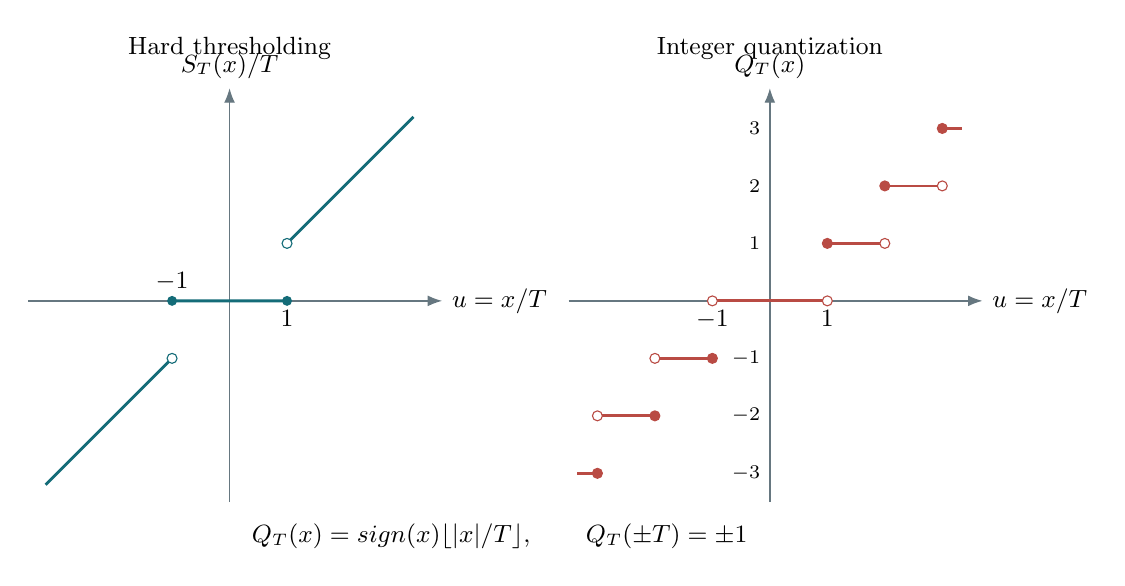
\begin{tikzpicture}[x=.73cm,y=.73cm]
\draw[axis] (-3.5,0)--(3.7,0) node[right] {$u=x/T$};\draw[axis] (0,-3.5)--(0,3.7) node[above] {$S_T(x)/T$};
\draw[curve] (-3.2,-3.2)--(-1,-1) (1,1)--(3.2,3.2) (-1,0)--(1,0);
\foreach \u/\v in {-1/-1,1/1}{\draw[accent,fill=white] (\u,\v) circle(1.8pt);}
\foreach \u in {-1,1}{\fill[accent] (\u,0) circle(1.8pt);}
\node at (0,4.4) {Hard thresholding};\node[above] at (-1,0) {$-1$};\node[below] at (1,0) {$1$};
\begin{scope}[shift={(9.4,0)}]
\draw[axis] (-3.5,0)--(3.7,0) node[right] {$u=x/T$};\draw[axis] (0,-3.5)--(0,3.7) node[above] {$Q_T(x)$};
\draw[signalred,line width=1pt] (-3.35,-3)--(-3,-3);
\draw[signalred,fill=signalred] (-3,-3) circle(1.8pt);
\draw[signalred,line width=1pt] (-3,-2)--(-2,-2);
\draw[signalred,fill=white] (-3,-2) circle(1.8pt);
\draw[signalred,fill=signalred] (-2,-2) circle(1.8pt);
\draw[signalred,line width=1pt] (-2,-1)--(-1,-1);
\draw[signalred,fill=white] (-2,-1) circle(1.8pt);
\draw[signalred,fill=signalred] (-1,-1) circle(1.8pt);
\draw[signalred,line width=1pt] (-1,0)--(1,0);
\draw[signalred,fill=white] (-1,0) circle(1.8pt);
\draw[signalred,fill=white] (1,0) circle(1.8pt);
\draw[signalred,line width=1pt] (1,1)--(2,1);
\draw[signalred,fill=signalred] (1,1) circle(1.8pt);
\draw[signalred,fill=white] (2,1) circle(1.8pt);
\draw[signalred,line width=1pt] (2,2)--(3,2);
\draw[signalred,fill=signalred] (2,2) circle(1.8pt);
\draw[signalred,fill=white] (3,2) circle(1.8pt);
\draw[signalred,line width=1pt] (3,3)--(3.35,3);
\draw[signalred,fill=signalred] (3,3) circle(1.8pt);
\foreach \k in {-3,-2,-1,1,2,3}{\node[left,font=\scriptsize] at (0,\k) {$\k$};}
\node at (0,4.4) {Integer quantization};\node[below] at (-1,0) {$-1$};\node[below] at (1,0) {$1$};
\end{scope}
\node at (4.7,-4.1) {$Q_T(x)=\operatorname{sign}(x)\lfloor|x|/T\rfloor,\qquad Q_T(\pm T)=\pm1$};
\end{tikzpicture}
\end{document}
